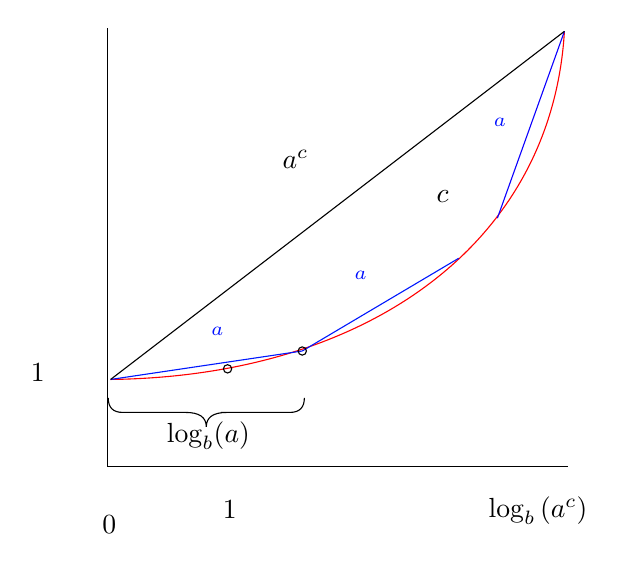
\begin{tikzpicture}[x=0.75pt,y=0.75pt,yscale=-1,xscale=1]
%uncomment if require: \path (0,300); %set diagram left start at 0, and has height of 300

%Curve Lines [id:da5666747848036192] 
\draw [color={rgb, 255:red, 255; green, 0; blue, 0 }  ,draw opacity=1 ]   (141.15,193.12) .. controls (265.44,191.62) and (353.8,127.23) .. (359.79,25.4) ;
%Straight Lines [id:da028560556373229073] 
\draw    (139.65,235.05) -- (361.28,235.05) ;
%Straight Lines [id:da8787938487899625] 
\draw    (139.65,23.9) -- (139.65,235.05) ;
%Straight Lines [id:da788769211427464] 
\draw [color={rgb, 255:red, 0; green, 24; blue, 253 }  ,draw opacity=1 ]   (141.15,193.12) -- (233.5,179.41) ;
%Straight Lines [id:da7332679005966856] 
\draw [color={rgb, 255:red, 12; green, 0; blue, 255 }  ,draw opacity=1 ]   (359.79,25.4) -- (327.5,115.41) ;
%Straight Lines [id:da7194926321605494] 
\draw    (141.15,193.12) -- (359.79,25.4) ;
%Straight Lines [id:da019397101725570853] 
\draw [color={rgb, 255:red, 0; green, 24; blue, 253 }  ,draw opacity=1 ]   (233.5,179.41) -- (308.87,134.72) ;
%Shape: Brace [id:dp6265659815745908] 
\draw   (140,202) .. controls (140,206.67) and (142.33,209) .. (147,209) -- (177.25,209) .. controls (183.92,209) and (187.25,211.33) .. (187.25,216) .. controls (187.25,211.33) and (190.58,209) .. (197.25,209)(194.25,209) -- (227.5,209) .. controls (232.17,209) and (234.5,206.67) .. (234.5,202) ;
%Shape: Circle [id:dp9573621524250069] 
\draw   (231.5,179.41) .. controls (231.5,178.31) and (232.4,177.41) .. (233.5,177.41) .. controls (234.6,177.41) and (235.5,178.31) .. (235.5,179.41) .. controls (235.5,180.51) and (234.6,181.41) .. (233.5,181.41) .. controls (232.4,181.41) and (231.5,180.51) .. (231.5,179.41) -- cycle ;
%Shape: Circle [id:dp3800718490662076] 
\draw   (195.5,188) .. controls (195.5,186.9) and (196.4,186) .. (197.5,186) .. controls (198.6,186) and (199.5,186.9) .. (199.5,188) .. controls (199.5,189.1) and (198.6,190) .. (197.5,190) .. controls (196.4,190) and (195.5,189.1) .. (195.5,188) -- cycle ;

% Text Node
\draw (322,248.5) node [anchor=north west][inner sep=0.75pt]    {$\log_{b}\left( a^{c}\right)$};
% Text Node
\draw (135.9,257.4) node [anchor=north west][inner sep=0.75pt]    {$0$};
% Text Node
\draw (101.46,184.02) node [anchor=north west][inner sep=0.75pt]    {$1$};
% Text Node
\draw (222.74,81.19) node [anchor=north west][inner sep=0.75pt]    {$a^{c}$};
% Text Node
\draw (188.49,166.87) node [anchor=north west][inner sep=0.75pt]  [font=\scriptsize,color={rgb, 255:red, 0; green, 15; blue, 255 }  ,opacity=1 ]  {$a$};
% Text Node
\draw (290,110.81) node [anchor=north west][inner sep=0.75pt]    {$\dotsc $};
% Text Node
\draw (297,100.81) node [anchor=north west][inner sep=0.75pt]    {$c$};
% Text Node
\draw (257.49,139.87) node [anchor=north west][inner sep=0.75pt]  [font=\scriptsize,color={rgb, 255:red, 0; green, 15; blue, 255 }  ,opacity=1 ]  {$a$};
% Text Node
\draw (324.49,65.87) node [anchor=north west][inner sep=0.75pt]  [font=\scriptsize,color={rgb, 255:red, 0; green, 15; blue, 255 }  ,opacity=1 ]  {$a$};
% Text Node
\draw (194,250.4) node [anchor=north west][inner sep=0.75pt]    {$1$};
% Text Node
\draw (167,212.4) node [anchor=north west][inner sep=0.75pt]    {$\log_{b}( a)$};


\end{tikzpicture}